\section{RQ2 and RQ3: Can the Benchmark Oracle See the Edit?}
\label{sec:oracle}

Whether a project's benchmarks can see a change to a function depends on three factors in turn.
The function must be \emph{executed} by some benchmark case (coverage, RQ2).
It must take a large enough \emph{share} of that case's time for a change to be \emph{visible} at the case level: a slowdown by a factor $f$ in a function with share $s$ changes the case by about $1+s(f-1)$, which is Amdahl's law applied to one benchmark case~\cite{amdahl1967validity}.
And the case-level effect must be \emph{detectable} above the measurement noise (power, RQ3).
None of these factors is new as a concept: Peass and Laaber and Leitner already separate uncovered changes from changes below the noise~\cite{reichelt2023peass,laaber2018evaluation}, and the share is an operationalisation of Amdahl's law that splits their ``below the noise'' case into a small effect and a noisy measurement.
What we add is a measurement of how often each factor bites for real optimization edits on one project.
Table~\ref{tab:oracle} lists the three factors per edit; the injected slowdowns at the end of this section test them.

\begin{table*}[t]
\caption{The benchmark oracle per agent-labelled optimization edit on networkx: number of benchmark cases whose $S_0$ profile executes a changed function; the largest share of a reaching case's time spent in the changed functions (cProfile at the edit's parent, approximate); and the expected case-level ratio $1+s(f-1)$ if the changed code were \PowFactorMid\x{} or \PowFactorHigh\x{} slower. Bold: above asv's factor of \AsvFactor{} at three decimals, so a flag is possible before noise is considered. ``--'': no case executes the edit.}
\label{tab:oracle}
\centering\footnotesize\setlength{\tabcolsep}{4pt}
% Generated by scripts/make_all.py (write_oracle_table). DO NOT EDIT.
\begin{tabular}{@{}rlrrrr@{}}
\toprule
Step & Changed function & Cases & Max share & Ratio at $1.2\times$ & Ratio at $2\times$ \\
\midrule
1 & \texttt{global\_parameters +1} & -- & -- & -- & -- \\
2 & \texttt{bidirectional\_dijkstra} & -- & -- & -- & -- \\
3 & \texttt{\_dijkstra\_multisource} & 8 & 0.864 & \textbf{1.173} & \textbf{1.864} \\
4 & \texttt{is\_connected +1} & 3 & 0.021 & 1.004 & 1.021 \\
5 & \texttt{\_single\_shortest\_path +2} & -- & -- & -- & -- \\
7 & \texttt{kruskal\_mst\_edges} & -- & -- & -- & -- \\
9 & \texttt{\_pagerank\_scipy +1} & 4 & 0.998 & \textbf{1.200} & \textbf{1.998} \\
10 & \texttt{\_build\_paths\_from\_predecessors} & 1 & 0.502 & 1.100 & \textbf{1.502} \\
11 & \texttt{DiGMState.\_\_init\_\_ +1} & -- & -- & -- & -- \\
12 & \texttt{edmonds\_karp\_impl +1} & -- & -- & -- & -- \\
14 & \texttt{\_build\_paths\_from\_predecessors} & 1 & 0.565 & \textbf{1.113} & \textbf{1.565} \\
15 & \texttt{lattice\_reference +1} & -- & -- & -- & -- \\
16 & \texttt{\_triangles\_and\_degree\_iter} & 4 & 0.999 & \textbf{1.200} & \textbf{1.999} \\
18 & \texttt{chain\_decomposition} & -- & -- & -- & -- \\
\bottomrule
\end{tabular}

\end{table*}
\TODO{Detectability per edit against each reaching case's measured noise floor needs $\sigma$ for those cases (only the flagged ones have it); add it as a column when available.}

\subsection{Executed: coverage of optimization edits (RQ2)}
\label{sec:rq2}

On networkx, for \BOneAgentUnreached{} of the \NxAgentOpt{} replayed optimization edits (\BOneAgentPct\pct, Wilson CI \ci{\BOneAgentLo}{\BOneAgentHi}), the measured profile of no benchmark case contains any function the edit changed (Fig.~\ref{fig:coverage}).
By static reach, \BOneAgentStatic{} of \NxAgentOpt{} are unreached (\BOneAgentStaticPct\pct, \ci{\BOneAgentStaticLo}{\BOneAgentStaticHi}).
With the earlier subject-only labels the counts are \BOneManualUnreached{} of \NxManualOpt{} (\BOneManualPct\pct, \ci{\BOneManualLo}{\BOneManualHi}) by profile and \BOneManualStatic{} of \NxManualOpt{} by static reach; over all \NxReplayed{} replayed edits they are \BOneAllUnreached{} and \BOneAllStatic{}.
The two label sets differ by one edit, which is unreached under both measures, so the reading does not depend on which of our two label sets is used.
Because every interval includes values below one half, we say that \emph{many} optimization edits on networkx are unreached, not most.

\begin{figure}[t]
\centering
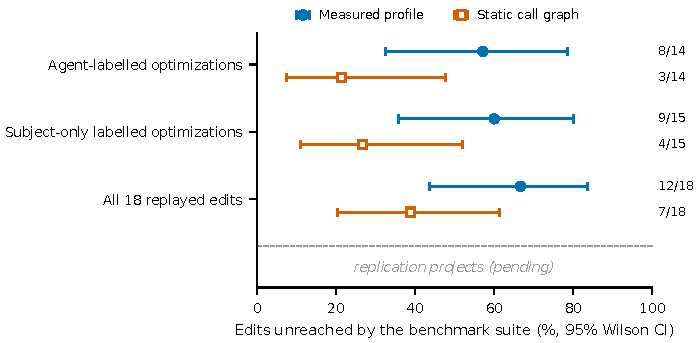
\includegraphics[width=\columnwidth]{figures/fig_coverage.pdf}
\caption{Share of replayed networkx edits that no benchmark executes, by measured profile and by static reach, with Wilson 95\pct{} intervals, for three edit sets. The replication rows are pending.}
\label{fig:coverage}
\end{figure}

\textbf{Reach at the base state.} Reach was measured with the $S_0$ suite and $S_0$ profiles.
A lookup of every changed function by qualified name found \ConstructUnreached{} edits unreached by construction: each has a changed function that exists at $S_0$, and all exist at their parent.
Profiles were still taken at $S_0$, not at each edit's parent, so a benchmark added upstream in between would be missed (Section~\ref{sec:threats}).
\TODO{Recompute with the upstream suite and profiles at each edit's parent, as the replication protocol does.}

\textbf{Static reach is not a bound.} Static reach leaves fewer edits unreached than the measured profile on every edit set, because the heavy benchmark module imports most of the package and a static graph connects it to functions it never calls; from an old base it can also miss functions added later (Appendix~\ref{app:q3}).
The motivating edit (step~2) is an example: static reach connects all \NxBenchCases{} cases to \texttt{bidirectional\_dijkstra}, and no profile executes it.
We therefore count reach by measured profile only.

\TODO{E1 (B1 replication): to meet the bar for the full paper, at least four to five projects and fifty to sixty labelled true optimizations pooled, with profiles at each edit's parent; per-project and pooled unreached shares with Wilson CIs as forest-plot rows in Fig.~\ref{fig:coverage}; attrition per the pre-registered rule; and the thesis restated or reframed by the pre-registered decision rule.}

\subsection{Visible: the changed function's share of a case}
\label{sec:share}

For the injected slowdowns, we estimated the share of each reaching case's time spent in the slowed function with cProfile at the slowdown's state (unpatched), as the function's inclusive time over the case's profiled time.
cProfile overhead inflates call-heavy code, so the shares are approximate.
For a slowdown that calls the function body twice, the expected case-level ratio is about one plus the share.

\textbf{A share miss.} \#3 (\texttt{is\_connected}) is executed by three profiled cases of the heavy module but takes only about \ShareThreeLo--\ShareThreeHi{} of their time, so doubling it should change them by a ratio of about \ExpThree; the observed ratios stayed near one.
asv's ratio condition (above \AsvFactor) can never flag such a change, however many samples are taken.
\#3 is therefore a miss of a diluted effect: executed by a benchmark is not the same as visible to it.

\textbf{Detections match the share.} For \#2 the share is \ShareTwoLo--\ShareTwoHi, which predicts ratios close to the observed \SlowTwoRatioLo--\SlowTwoRatioHi.
For \#8 the share is \ShareEight, but its slowdown changes one membership test inside the function rather than doubling the body, so one plus the share does not predict its ratio.
\textbf{Per optimization edit.} We computed the same share for every agent-labelled optimization edit, at the edit's parent state, as the largest share of any reaching case's time spent in the changed functions (Table~\ref{tab:oracle}).
Of the \NxAgentOpt{} edits, \BOneAgentUnreached{} are executed by no benchmark; one (step~4) is executed but diluted, with a share of \EditShareDiluted, so even a doubling of its code would move its benchmarks by about two percent; and the others have large shares (\EditShareBigLo--\EditShareBigHi).
If the changed code were \PowFactorMid\x{} slower, at most \EditsClearMid{} of the \NxAgentOpt{} edits would move a benchmark past asv's factor at all, before noise is considered; one more (step~10) sits at the factor, and because the cProfile share is approximate (to about a hundredth), it cannot be classified either way. At \PowFactorHigh\x, \EditsClearHigh{} would.
These are expected effects from approximate shares, not detections; the noise floor below decides which of them a run would flag.

\subsection{Detectable: noise and power (RQ3)}
\label{sec:rq3}

In the A/A control, asv's rule gave \AAFalse{} false verdicts in \AAComparisons{} per-repeat comparisons (Wilson upper bound \AAUpper\pct); the \AAComparisons{} comparisons are the same \AACases{} cases twice, so the bound is optimistic.
The noise sits near the threshold: some cases passed the $p$ condition and stayed ``same'' only on the ratio condition, and under a fixed run order one case reached a ratio of \AAMaxSameRatio{} without passing the $p$ condition.
\textbf{The pre-registered floor.} For every case with a slower verdict we ran an A/A at the verdict's own state and protocol, \SigmaRepeats{} repeats with the order rotated, and applied the pre-registered rule: a verdict survives if its ratio exceeds $1+3\sigma$, with $\sigma$ the standard deviation of the per-repeat A/A ratios.
Only \#2's on-target verdicts survive (all \SlowTwoCases{} cases, also under a bootstrap $\sigma$).
\#8's case has a floor of \FloorEight, so it cannot detect a slowdown of the size injected; its own A/A run even returned ``slower'' (pooled ratio \EightAAPooled), so its original verdict is indistinguishable from noise.
\#1's off-target case (floor \FloorOne) and the profile-completeness flag for \#9 (\SlowNineRatio\x{} against a floor of \FloorNine) do not survive either.
With five repeats, each $\sigma$ has four degrees of freedom, so every floor is uncertain; \#2's margin is large, while \#9 sits at its floor.
\TODO{E2 remainder: $\sigma$ for the other benchmark cases (none outside the flagged ones has it), and a larger heavy-module A/A sample of at least ten seeded cases.}

\textbf{Power at the verdict design.} We bootstrapped detection probability from the A/A samples at the verdict design (\VerdictSamples{} pooled samples per side, exact test) under asv's rule plus the pre-registered floor.
At a slowdown of \PowFactorMid\x, the median detection probability is \PowDesignAllMid{} over all A/A cases, but only \PowDesignAlgoMid{} for the \AAAlgoCases{} sampled cases of the heavy module (\PowDesignAlgoMidBoot{} with a bootstrap $\sigma$; \PowDesignAlgoMidNoFloor{} without the floor); at \PowFactorOneFive\x{} it is \PowDesignAlgoOneFive{} and at \PowFactorHigh\x{} \PowDesignAlgoTwo{} for those cases.
So once the floor applies, the module that holds most of the cost reliably detects only slowdowns of about \PowFactorOneFive\x{} or more.
This rests on \AAAlgoCases{} of its \NxAlgoCases{} cases and on $\sigma$ from two A/A repeats, and the bootstrap ignores the structure between processes and repeats, so the values are optimistic and indicative, not a module-wide estimate.
Fig.~\ref{fig:power} shows the earlier bootstrap at the A/A design (fifteen samples per side, no floor), which gives \PowAllOneTwo{} and \PowAlgoOneTwo{} at \PowFactorMid.

\begin{figure}[t]
\centering
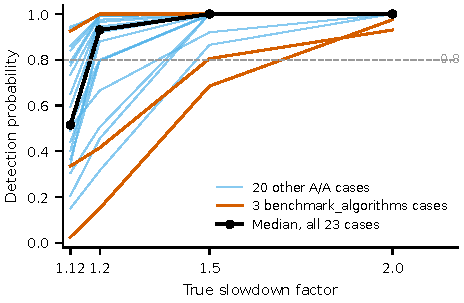
\includegraphics[width=\columnwidth]{figures/fig_power.pdf}
\caption{Bootstrap detection probability of asv's rule under the exact Mann-Whitney test, by slowdown factor, for the A/A cases on networkx. The heavy-module curve rests on three sampled cases.}
\label{fig:power}
\end{figure}

\subsection{Injected slowdowns as the test}
\label{sec:slowdowns}

\textbf{Pre-registered primary result.} Regression safety of reduced benchmark selection is \emph{not measurable} on networkx with the frozen slowdown set: no slowdown was detected on target within the pre-registered strength bands, so the regression set that selection arms were to be judged on is empty.
This is partly a consequence of the bands: the on-target ratios of \#2 (\SlowTwoRatioLo--\SlowTwoRatioHi\x) fall in the gap between the moderate band's upper end (\BandModHi\x) and the strong band (twofold), and \#8 (\SlowEightRatio\x) falls below the moderate band.

\textbf{Detection.} Fig.~\ref{fig:slowdowns} classifies the \NumSlowdowns{} slowdowns.
One rule decides all flags: a flag counts as a detection only if the flagged case executes the slowed function in its profile; other flags are reported as off target.
Within reach, each verdict compares \VerdictSamples{} pooled samples per side.
Slowdown \#$k$ sits in the function changed at one replay step: \#0--\#5 at steps one to six and \#6--\#9 at steps eight to eleven.
Under asv's rule the full suite flags \SlowDetClassified{} slowdowns (Wilson \ci{\SlowDetClassLo}{\SlowDetClassHi}), \SlowDetOnTarget{} of them on target (\ci{\SlowDetOnTargetLo}{\SlowDetOnTargetHi}); above the pre-registered noise floor it detects \FloorDetect{} (\ci{\FloorDetectLo}{\FloorDetectHi}).
\#2 (\texttt{\_dijkstra\_multisource}) is flagged by all \SlowTwoCases{} profiled cases at \SlowTwoRatioLo--\SlowTwoRatioHi\x, far above their floors; \#8 (\texttt{\_build\_paths\_from\_predecessors}) is flagged by its one profiled case at \SlowEightRatio\x, below that case's floor of \FloorEight.
\#1's only flag (\SlowOneRatio\x, exact $p=\SlowOneExactP$) is on a case that never executes \texttt{bidirectional\_dijkstra}, whose body is the only code the patch changes; we classify it as an off-target flag, and it does not pass its floor either.
Across the oracle, \OffTargetVerdictable{} off-target comparisons could yield a verdict (plus fifty spot-check comparisons that cannot, \OffTargetComparisons{} in all); \OffTargetObserved{} of them gave a non-``same'' verdict.
At the nominal $\alpha=\AsvAlpha$ about \OffTargetExpected{} would be expected, but the null rate of the joint rule is not calibrated here (samples within a process are correlated, the comparisons share cases, and the ratio condition and the discreteness of the exact test pull the other way), so we report the off-target flags descriptively rather than as consistent with chance; the repeat below found off-target flips on about \TwoFlipPct\pct{} of cases in this fixed-directory design.

\begin{figure}[t]
\centering
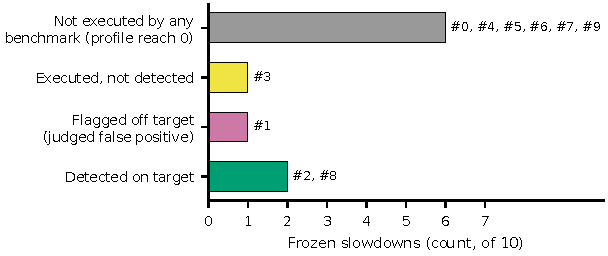
\includegraphics[width=\columnwidth]{figures/fig_slowdowns.pdf}
\caption{The frozen slowdowns on networkx by outcome under the full suite: not executed by any benchmark in its measured profile (coverage miss), executed but not detected, detected on target, and flagged off target.}
\label{fig:slowdowns}
\end{figure}

\textbf{Misses by factor.} Static reach does not separate these slowdowns: the $S_0$ static call graph connects all \NxBenchCases{} cases to each of \#1--\#4 and \#8, so we classify by measured profile only (no case for \#1 and \#4, three for \#3, \SlowTwoCases{} for \#2, one for \#8).
We count a slowdown as missed when it is not detected on target, so \#1, flagged only off target, is missed.
Of the \SlowUndetected{} missed slowdowns, \SlowUnreachedProfile{} lie in functions that no measured profile executes (\SlowMissedUnreached{} of them unreached by static reach as well, plus \#1 and \#4), and \#3 is the share miss above.
Because the slowdowns were placed in functions changed at their step, these counts follow from the reach of those functions; they check the profiles and the share argument, and are not an independent rate.
Under the pre-registered floor, \#8 is missed as well, and it is the one power miss in this set: its slowed function takes about half of its case's time, but that case's noise is too high (floor \FloorEight) for the effect to be distinguished.

\textbf{What this says about selection.} On this protocol, no selection among these benchmark cases can detect a slowdown that running all of them misses; with the same time budget, a selected subset could be run with more repetitions and gain power, which we did not test.
A check of the profiles' completeness (Appendix~\ref{app:completeness}) found one flag outside the measured reach, which neither passes its noise floor nor reproduced in a post-hoc re-check.

\textbf{Repeatability.} We repeated the oracle on the verdict-relevant cases of \#1, \#2, \#3 and \#8 at each slowdown's own state, with four repeats in alternating order (\RepSamples{} pooled samples per side, \RepRuns{} runs).
\RepAgree{} of \RepTotal{} verdicts agree with the original.
\#2's on-target verdicts repeat on all \SlowTwoCases{} cases at \RepTwoLo--\RepTwoHi\x.
The two off-target flags (\#1, and \#2's off-target case) do not repeat and are now ``same'', consistent with noise.
\#8 is again ``slower'' pooled (\RepEightRatio\x), but each order-balanced pair is ``same'', the ratio is far below its floor, and the same case's A/A also returned ``slower'', so the agreement carries no evidence of a real effect.
\#3 is ``same'' on all three cases, which is no evidence of an effect at this protocol; on one case a moderate effect is not excluded.
Detection above the floor therefore stays at \FloorDetect{} of \NumSlowdowns, a result the repeat checks only for \#1, \#2, \#3 and \#8.
\#1's block was interrupted by a time cap and resumed hours later, so its second order-balanced pair mixes runs from two sessions; its ratio matches the first pair.
A second tier repeated the off-target cases of all five reached slowdowns with two order-balanced repeats; for \#2, \#3 and \#4 each side kept one clone directory, as in the original oracle.
Of \TwoTotal{} off-target verdicts, \TwoAgree{} again read ``same'' and \TwoFlips{} (\TwoFlipPct\pct, Wilson \ci{\TwoFlipLo}{\TwoFlipHi}, too narrow because cases share runs) became non-``same'', against about \TwoExpected{} expected at the nominal level; that nominal level assumes exchangeable samples, which pooled runs from few processes are not.
\TwoFaster{} of these flips are ``faster'', which a patch that only adds work cannot cause.
In every A/B run, including the original oracle, the unpatched side ran in one clone directory and the patched side in another, so the edit and the clone directory are confounded.

\textbf{Identical code.} To test whether such flips need an edit at all, we ran the same tier-2 cases and design with identical, unpatched code in the two clone directories.
\DirAANonSame{} of \DirAATotal{} cases still returned a non-``same'' verdict (\DirAAPct\pct, Wilson \ci{\DirAALo}{\DirAAHi}), a rate the intervals cannot distinguish from the \TwoFlipPct\pct{} with the patches, and only \DirAARecur{} of the \DirAARecurN{} earlier flips at that state recurred.
So the off-target flips need no effect of the edit.
This control also kept one directory per side, so for \#8 and \#1 we swapped the directories between the two repeats, balancing the edit across directories (and, with it, run order).
The swap did not remove the flips: \SwapFlips{} of \SwapTotal{} off-target verdicts (\SwapPct\pct) became non-``same'', and none reversed its sign when the directories swapped, so a directory effect alone does not produce them.
Nor do they show a stable effect of the edit: of the \CrossNightN{} \#8 cases that could be compared with an earlier night under the same setup, only \CrossNightAgree{} reproduced, and sign consistency across repeats is expected after selecting on a small pooled $p$ (the identical-code flips kept their sign too).
Their cause, per-night variation, an anti-conservative test on correlated samples, or an effect specific to a few sensitive cases (one \texttt{connected\_components} case flags under two unrelated slowdowns), is unresolved, and we could not test machine load.
In this design, then, single A/B verdicts up to about \DirAAMaxDev\x{} in either direction, the largest deviation seen with identical code, are not evidence of an edit effect; at the tier-2 sample size, about \DirAAFalsePerComp{} false changes (\DirAAFalseLo--\DirAAFalseHi) are expected per comparison of all \NxBenchCases{} cases, assuming independent cases.
This covers \#8 (\SlowEightRatio--\RepEightRatio\x), all off-target flags and the profile-completeness flag.
\#2's on-target ratios (\RepTwoLo--\RepTwoHi\x) lie well above it, cleared their own noise floors and repeated, so \#2 stands as the one detection.
The swapped run repeated only off-target cases, so \#8's on-target verdict was not re-tested with swapped directories.

\paragraph*{Answers to RQ2 and RQ3}
On networkx, the project's own benchmarks execute none of the changed functions for many optimization edits (\BOneAgentUnreached{} of \NxAgentOpt{}, CI \ci{\BOneAgentLo}{\BOneAgentHi}); for those, full benchmarking cannot confirm the speed-up or see a slowdown in the changed functions, as far as one profile shows (RQ2).
Where a benchmark does execute the changed code, its share and the noise decide (RQ3): above the pre-registered floor the full suite detected \FloorDetect{} of \NumSlowdowns{} injected slowdowns, the one whose function dominates its cases; one slowdown was hidden by a small share and one by noise; and per edit, at most \EditsClearMid{} of the \NxAgentOpt{} optimization edits could show a \PowFactorMid\x{} slowdown of their changed code at all.
